\subsection{Comparing the Worst-Case and Average-Case Approximations}
\label{worst-vs-avg}

\iffalse
In this section, we show that the the results of Section
\ref{fixed-degree} that hold in expectation also hold in the worst
case with high probability using concentration bounds. We can convert
the expectation results to a lower bound that holds with high
probability using concentration results like Chernoff bounds. While
Chernoff bounds are usually stated for independent variables, the
variant below holds for any number pairwise non-positively correlated
variables.

\begin{thm}
Let $X_1,\ldots, X_n$ be non-positively correlated variables. If $X=\sum_{i=1}^n X_i$, then for any $\delta\geq 0$
\[ Pr[X \geq (1+\delta)\E[X] ] \leq \left(\frac{e^\delta}{(1+\delta)^{1+\delta}}\right)^{\E[X]} \]
\end{thm}

Now note that the variables $1-X_v$ for each $v\in R$ are
non-positively correlated. In particular, if $N(v)$ and $N(v')$ are
disjoint, then $1-X_v$ and $1-X_{v'}$ are independent. Otherwise, $v$
not claiming any edges can only increase the probability that $v'$
gets an edge from any vertex $u\in N(v)\cap N(v')$, so the variables
would be negatively correlated. Setting $\delta=1$ in the
theorem above now proves the following:

\begin{thm}
The random sampling algorithm produces a solution of size at least $r(1-2\exp(-ck))$ with probability at least $1-(e/4)^{r\exp(-ck)}$.
\end{thm}

That is, the probability of producing a constant factor approximation decreases exponentially with $r$.

With these high probability bounds in place, i
\fi

It is instructive to compare the performance of the random sampling
algorithm with that of greedy. 
%Arda: Your high prob bound is for 1 - 2\exp(-ck) and not for (1 - exp(ck)) so why aren't you using the 2-version in the ratio below?
With high probability, the approximation ratio of the
randomized algorithm is $(1-\exp(-ck))/(1-\exp(-dk))$ while the
approximation ratio of the greedy algorithm is always at least
$1/2$. In the following graphs $f\geq 1$ represents a value such that
$d=fc$ and we use the values $k=0.1$ and $k=0.2$ respectively since
the case that is practical for our purposes is when $l \ll r$. In the
graphs below, the red curve shows the approximation ratio for the
model used in Section \ref{fixed-degree} and the blue curve shows the
worst case approximation ratio described in section 5. As we would
expect, the sampling algorithm performs outperforms the greedy
algorithm significantly when $k$ and more importantly $c$ gets larger.

\begin{figure}[h]
\begin{minipage}[h]{0.45\linewidth}
\centering
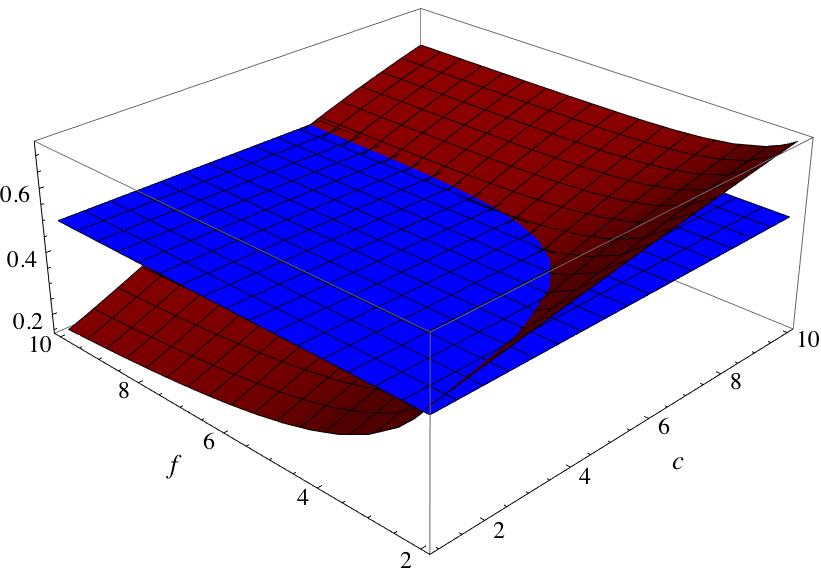
\includegraphics[width=\textwidth]{k=0_1.png}
\caption{Approximation ratios when $k$=0.1}
\end{minipage}
\hspace{0.5cm}
\begin{minipage}[h]{0.45\linewidth}
\centering
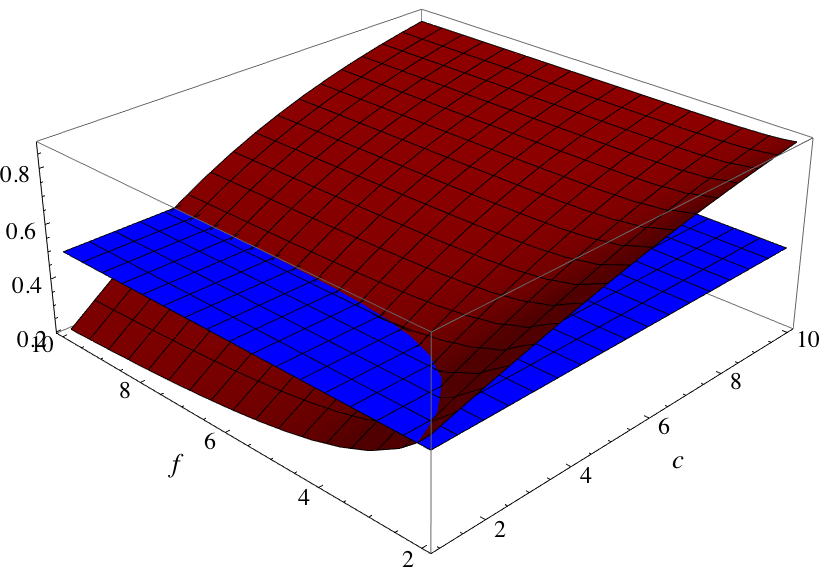
\includegraphics[width=\textwidth]{k=0_2.png}
\caption{Approximation ratios when $k$=0.2}
\end{minipage}
\end{figure} 
